\documentclass[portrait, color=UCLburgundy, margin=1cm]{uclposter}

\newcommand{\boldf}{\bm{f}}
\newcommand{\boldmu}{\bm{\mu}}
\newcommand{\boldalpha}{\bm{\alpha}}
\newcommand{\boldr}{\bm{r}}
\newcommand{\boldt}{\bm{t}}
\newcommand{\boldg}{\bm{g}}
\newcommand{\boldtheta}{\bm{\theta}}

% Warping operators
\newcommand{\MPWarp}{\tilde{\mathcal{W}}}
\newcommand{\Warp}{\mathcal{W}}

% Others
\newcommand{\etal}{\textit{et al.}~}
\newcommand{\ie}{i.e., }
\newcommand{\eg}{e.g., }

\usepackage{bm}
\usepackage{algorithm}
\usepackage{algorithmic}
\usepackage{caption}
\usepackage{blindtext}
\usepackage{siunitx}

\usepackage[acronym, nomain]{glossaries}

% Define "long-s" key: 
\glsaddkey* {longs}% key 
{\glsentrylong{\glslabel}s}% default value 
{\glsentrylongs}% command analogous to \glsentrytext 
{\Glsentrylongs}% command analogous to \Glsentrytext 
{\glslongs}% command analogous to \glstext 
{\Glslongs}% command analogous to \Glstext 
{\GLSlongs}% command analogous to \GLStext

%% Define "short-s" key: 
\glsaddkey* {shorts}% key 
{\glsentryshort{\glslabel}s}% default value 
{\glsentryshorts}% command analogous to \glsentrytext 
{\Glsentryshorts}% command analogous to \Glsentrytext 
{\glsshorts}% command analogous to \glstext 
{\Glsshorts}% command analogous to \Glstext 
{\GLSshorts}% command analogous to \GLStext

\DeclareRobustCommand{\glss}[1]
{%
  \ifglsused{#1}{\glsshorts{#1}}{\glslongs{#1} (\glsshorts{#1})\glsunset{#1}}%
}

\DeclareRobustCommand{\Glss}[1]
{%
  \ifglsused{#1}{\Glsshorts{#1}}{\Glslongs{#1} (\glsshorts{#1})\glsunset{#1}}%
}

\newacronym{18F-FDG}{18F-FDG}{Fluorine-$18$ Fludeoxyglucose}
\newacronym{1D}{1D}{$1$-Dimensional}
\newacronym{2D}{2D}{$2$-Dimensional}
\newacronym{3D}{3D}{$3$-Dimensional}
\newacronym[longs={$3$-Dimensional Point Clouds}, shorts={3DPCs}]{3DPC}{3DPC}{$3$-Dimensional Point Cloud}
\newacronym{4D}{4D}{$4$-Dimensional}
% \newacronym{4DCT}{4DCT}{$4$-Dimensional Computed Tomography}
\newacronym{4DCT}{4DCT}{$4$D Computed Tomography}
\newacronym{AC}{AC}{Attenuation Corrected}
\newacronym{AD}{AD}{Affine Deformation}
\newacronym{AP}{AP}{Anterior Posterior}
\newacronym{ATP}{ATP}{Adenosine Triphosphate}
% \newacronym{AV-CCT}{AV-CCT}{Averaged CINE-Computed Tomography}
\newacronym{AV-CCT}{AV-CCT}{Averaged CINE-CT}
\newacronym{BE}{BE}{Bending Energy}
\newacronym{BFGS}{BFGS}{Broyden Fletcher Goldfarb Shanno}
\newacronym{CC}{CC}{Correlation Coefficient}
% \newacronym{CCT}{CCT}{CINE-Computed Tomography}
\newacronym{CCT}{CCT}{CINE-CT}
\newacronym{CG}{CG}{Conjugate Gradient}
\newacronym{COM}{COM}{Centre of Mass}
\newacronym[longs={Control Points}, shorts={CPs}]{CP}{CP}{Control Point}
\newacronym[longs={Control Point Grids}, shorts={CPGs}]{CPG}{CPG}{Control Point Grid}
\newacronym{CT}{CT}{Computed Tomography}
\newacronym{DDG}{DDG}{Data Driven Gating}
\newacronym{DD-PCA}{DD-PCA}{Data Driven Principal Component Analysis Surrogate Signal Extraction}
\newacronym{DD}{DD}{Data Driven}
\newacronym{DIP}{DIP}{Deep Image Prior}
\newacronym[longs={Deformation Vector Fields}, shorts={DVFs}]{DVF}{DVF}{Deformation Vector Field}
\newacronym{DWB}{DWB}{Dynamic Whole Body}
\newacronym{EANM}{EANM}{European Association of Nuclear Medicine}
\newacronym{EM}{EM}{Expectation Maximisation}
\newacronym{FDG}{FDG}{Fluorodeoxyglucose}
\newacronym{FFT}{FFT}{Fast Fourier Transform}
\newacronym[longs={Fields of View}, shorts={FOVs}]{FOV}{FOV}{Field Of View}
\newacronym{FWHM}{FWHM}{Full Width at Half Maximum}
\newacronym{GAN}{GAN}{Generative Adversarial Networks}
\newacronym{GD}{GD}{Gradient Descent}
\newacronym{GE}{GE}{General Electric}
\newacronym{GPU}{GPU}{Graphics Processing Unit}
\newacronym{GT}{GT}{Ground Truth}
\newacronym{HU}{HU}{Hounsfield Unit}
\newacronym[longs={Image Registrations}, shorts={IRs}]{IR}{IR}{Image Registration}
\newacronym{KBq/mL}{KBq/mL}{Kilo Becquerel per Millilitre}
\newacronym{KeV}{KeV}{Kilo Electron Volt}
\newacronym{KRG}{KRG}{Kinetic Respiratory Gating}
\newacronym{KV}{KV}{Kilo Volt}
\newacronym{L-BFGS-B}{L-BFGS-B}{Low memory Broyden Fletcher Goldfarb Shanno Bounded}
\newacronym{L-BFGS}{L-BFGS}{Low memory Broyden Fletcher Goldfarb Shanno}
\newacronym[longs={Light Emitting Diodes}, shorts={LEDs}]{LED}{LED}{Light Emitting Diode}
\newacronym{LE}{LE}{Linear Energy}
\newacronym{LR}{LR}{Linear Regression}
\newacronym[longs={Lines of Response}, shorts={LORs}]{LOR}{LOR}{Line of Response}
\newacronym{MAE}{MAE}{Mean Absolute Error}
\newacronym{MAD}{MAD}{Median Absolute Difference}
\newacronym{MAPE}{MAPE}{Mean Absolute Percentage Error}
\newacronym{MBF}{MBF}{Myocardial Blood Flow}
\newacronym{MCIR}{MCIR}{Motion Compensated Image Reconstruction}
\newacronym[longs={Motion Compensated Images}, shorts={MCIs}]{MCI}{MCI}{Motion Compensated Image}
\newacronym{MC}{MC}{Motion Correction}
\newacronym{MIC}{MIC}{Medical Imaging Convention}
\newacronym{MI}{MI}{Mutual Information}
% \newacronym{ML}{ML}{Maximum Likelihood}
\newacronym{ML}{ML}{Machine Learning}
\newacronym{MLAA}{MLAA}{Maximum Likelihood Reconstruction of Activity and Attenuation}
\newacronym{MLE}{MLE}{Maximum Likelihood Estimation}
\newacronym{MLEM}{MLEM}{Maximum Likelihood Expectation Maximisation}
\newacronym[longs={Motion Models}, shorts={MMs}]{MM}{MM}{Motion Model}
\newacronym{MPI}{MPI}{Myocardial Perfusion Imaging}
\newacronym{MR}{MR}{Magnetic Resonance}
\newacronym{MSc}{MSc}{Master of Science}
\newacronym{MSE}{MSE}{Mean Squared Error}
\newacronym[longs={Attenuation Maps}, shorts={Mu-Maps}]{Mu-Map}{Mu-Map}{Attenuation Map}
\newacronym{NAC}{NAC}{Non-Attenuation Corrected}
\newacronym{NMI}{NMI}{Normalised Mutual Information}
\newacronym{ND}{ND}{$n$-Dimensional}
\newacronym{NMC}{NMC}{Non-Motion Corrected}
\newacronym{NN}{NN}{Neural Network}
\newacronym{NRD}{NRD}{Non-Rigid Deformation}
\newacronym{NTOF}{NTOF}{Non-Time-of-Flight}
\newacronym{OSEM}{OSEM}{Ordered Subset Expectation Maximisation}
\newacronym[longs={Principal Components}, shorts={PCs}]{PC}{PC}{Principal Component}
\newacronym{PCA}{PCA}{Principal Component Analysis}
\newacronym{PCC}{PCC}{Pearson Correlation Coefficient}
\newacronym{PET}{PET}{Positron Emission Tomography}
\newacronym{PLL}{PLL}{Poisson Log Likelihood}
\newacronym{PSD}{PSD}{Power Spectral Density}
\newacronym{PSMA}{PSMA}{Prostate Specific Membrane Antigen}
\newacronym{RANSAC}{RANSAC}{Random Sample Consensus}
\newacronym{RCM}{RCM}{Respiratory Correspondence Model}
\newacronym{RD}{RD}{Rigid Deformation}
\newacronym{RDP}{RDP}{Relative Difference Prior}
\newacronym{RM}{RM}{Respiratory Motion}
\newacronym{RMC}{RMC}{Respiratory Motion Correction}
\newacronym{RMSE}{RMSE}{Root Mean Square Error}
\newacronym[longs={Regions of Interest}, shorts={ROIs}]{ROI}{ROI}{Region of Interest}
\newacronym{RPM}{RPM}{Real Time Position Management}
\newacronym{RTPM}{RTPM}{Real Time Position Management}
\newacronym{SAM}{SAM}{Spectral Analysis Method}
\newacronym{SGD}{SGD}{Stochastic Gradient Descent}
\newacronym{SI}{SI}{Superior Inferior}
\newacronym{SIRF}{SIRF}{Synergistic Image Reconstruction Framework}
\newacronym{SNR}{SNR}{Signal to Noise Ratio}
\newacronym[longs={Surrogate Signals}, shorts={SSs}]{SS}{SS}{Surrogate Signal}
\newacronym{SSD}{SSD}{Sum of Squared Differences}
\newacronym{SSIM}{SSIM}{Structural Similarity Index Measure}
\newacronym{STFT}{STFT}{Short-time Fourier transform}
\newacronym{STIR}{STIR}{Software for Tomographic Image Reconstruction}
\newacronym{SUV}{SUV}{Standard Uptake Value}
\newacronym{SVD}{SVD}{Singular Value Decomposition}
\newacronym[longs={Time Activity Curves}, shorts={TACs}]{TAC}{TAC}{Time Activity Curve}
\newacronym{TOF}{TOF}{Time-of-Flight}
\newacronym{TPS}{TPS}{Thin Plate Spline}
\newacronym{TV}{TV}{Total Variation}
\newacronym[longs={Volumes of Interest}, shorts={VOIs}]{VOI}{VOI}{Volume of Interest}
\newacronym{XCAT}{XCAT}{$4$-Dimensional Extended Cardiac Torso}

% \glsunset{18F-FDG}
% \glsunset{1D}
% \glsunset{2D}
% \glsunset{3D}
% \glsunset{4D}
% \glsunset{4DCT}
% \glsunset{ATP}
% \glsunset{BFGS}
% \glsunset{CT}
% \glsunset{EANM}
% \glsunset{FDG}
% \glsunset{GE}
% \glsunset{L-BFGS-B}
% \glsunset{L-BFGS}
% \glsunset{LED}
% \glsunset{MIC}
% \glsunset{MLAA}
% \glsunset{MLEM}
% \glsunset{MR}
% \glsunset{MSc}
% \glsunset{Mu-Map}
% \glsunset{NTOF}
% \glsunset{OSEM}
% \glsunset{PCA}
% \glsunset{PET}
% \glsunset{RANSAC}
% \glsunset{RPM}
% \glsunset{RTPM}
% \glsunset{SIRF}
% \glsunset{STIR}
% \glsunset{SUV}
% \glsunset{TOF}
% \glsunset{XCAT}


\usepackage[style=ieee, maxbibnames=1, minbibnames=1, maxcitenames=1, mincitenames=1, backend=biber, defernumbers=false]{biblatex}
\addbibresource{./Biblio.bib}
\addbibresource{./extraBib.bib}

\AtEveryBibitem{\clearfield{month}}
\AtEveryBibitem{\clearfield{day}}
\AtEveryBibitem{\clearfield{volume}}
\AtEveryBibitem{\clearfield{issue}}
\AtEveryBibitem{\clearfield{pages}}
\AtEveryBibitem{\clearfield{number}}
\AtEveryBibitem{\clearfield{title}}
\AtEveryBibitem{\clearfield{isbn}}
\AtEveryBibitem{\clearfield{keywords}}
\AtEveryBibitem{\clearfield{issn}}
\AtEveryBibitem{\clearfield{journal}}

\usepackage{fontspec}
\setmainfont[Ligatures=TeX]{LexendDeca-Regular.ttf}

\begin{document}
    \title{Pseudo-Bayesian DIP Denoising as a Preprocessing Step for Kinetic Modelling in Dynamic PET}
    
    \author[12*]{Alexander~C.~Whitehead}
    \author[1]{Kjell~Erlandsson}
    \author[3]{Ander~Biguri}
    \author[4]{Scott~D.~Wollenweber}
    \author[2]{\newline~Jamie~R.~McClelland}
    \author[12]{Kris~Thielemans}
    
    \affil[1]{INM, UCL}
    \affil[2]{CMIC, UCL}
    \affil[3]{University of Cambridge}
    \affil[4]{GE Healthcare}
    \affil[*]{alexander.whitehead.18@ucl.ac.uk}
    
    \maketitle

    \begin{multicols}{2}
        \section*{Introduction}
            \begin{highlightbox}[UCLlightgreen]
                \begin{itemize}
                    \item \gls{DIP} is a neural network based image denoising method where training and inference are performed independently on each new image~\cite{Ulyanov2018DeepPrior}.
                    \item For \acrshort{PET}, in~\cite{Gong2019PETPrior} a U-Net with relatively high count/low motion brain scans are used.
                    \item In~\cite{Hashimoto20214DNetwork}, \gls{DIP} is extended to \acrshort{4D} dynamic \acrshort{PET}. Multiple output branches are added, one for each dynamic time point.
                    \item This work seeks to extend or simplify previous work, in order to denoise \acrshort{4D} dynamic \acrshort{PET} data.
                \end{itemize}
            \end{highlightbox}
        
        \section*{Methods}
            \subsection*{\underline{\textbf{Overall flow}}}
                \begin{enumerate}
                    \item Reconstruct each time frame.
                    \item Denoise dynamic images method using modified \gls{DIP}, which also outputs uncertainty estimates.
                    \item Weighted indirect Patlak estimation used to generate Ki images~\cite{patlak1983GraphicalEvaluationBloodtoBrain}.
                \end{enumerate}
            
            \subsection*{\underline{\textbf{Network Design and Execution used for \gls{DIP}}}}
                \begin{itemize}
                    \item Modified U-Net~\cite{Weng2015U-Net:Segmentation}, with 7 down/upsampling stages (details in proceedings).
                    % \item Each down/upsampling block was preceded by 2 convolutional layers% (with two, four, eight, 16, 32, 64, or 128 channels).
                    % \item Split strided convolution and maxpooling downsampling layers concatenated. Trilinear upsampling layer.
                    % \item Edge padding, group normalisation~\cite{Wu2018GroupNormalization}, MISH activation~\cite{Misra2020Mish:Function}, and spatial dropout.
                    \item Spatial dropout to approximate Bayesian inference~\cite{Gal2015DropoutLearning}.
                    % \item Input data edge padded to the nearest power of two and standardised.
                    % \item Input to \gls{NN} summed with equal magnitude Gaussian noise.
                    \item Loss functions: \acrlong{MSE} and \acrshort{TV};  AdamW~\cite{Loshchilov2017DecoupledRegularization} optimiser.
                    \item 2 training regimes:
                    
                    \begin{enumerate}
                        \item Each time point was treated independently.
                        \item An independent model was updated for each time point, the mean of all model weights was then used to initialise the next iteration.
                    \end{enumerate}
                    
                    \item Training continued for all methods until the gradient of the loss function reduced below a threshold.
                \end{itemize}
            
            \subsection*{\underline{\textbf{\acrshort{PET} Acquisition Simulation and Image Reconstruction}}}
                \begin{itemize}
                    \item Dynamic scans were generated using \acrshort{XCAT}.
                    \item Patient-derived kinetic parameters were assigned to; 64 tissues, three tumours of 1.0cm diameter in the left lung, and three tumours of 2.5cm, 2.0cm and 1.0cm diameter in the liver.
                    \item An input function for \acrshort{18F-FDG}, taken from~\cite{langsjoEffectsSubanestheticKetamine2004}, was used to simulate \glss{TAC} to create dynamic images.
                    \item Reconstructed using \acrshort{OSEM} with 10 full iterations and 17 subsets.
                \end{itemize}
            
            \subsection*{\underline{\textbf{Kinetic Modelling}}}
                \begin{itemize}
                    \item Indirect Patlak estimation used to generate Ki images~\cite{patlak1983GraphicalEvaluationBloodtoBrain}.
                    \item The uncertainties of the parameters were estimated as follows:
                    
                    \begin{enumerate}
                        \item Normally distributed noise was added to the dynamic images, with standard deviation given by the \gls{DIP}-uncertainty.
                        \item Patlak analysis was performed.
                        \item The procedure was repeated for 10 noise realisations.
                        \item The standard deviation of the Ki parameters were calculated.
                    \end{enumerate}
                \end{itemize}
            
            \subsection*{\underline{\textbf{Evaluation}}}
                \begin{itemize}
                    \item Data were also denoised using \acrshort{TV}, and the \gls{DIP} method presented in~\cite{Gong2019PETPrior}.
                    \item Comparisons used included: A visual analysis, \acrshort{SSIM} to the ground truth~\cite{Wang2009MeanMeasures}, and Ki values.
                \end{itemize}
        
        \section*{Conclusion}
            \begin{highlightbox}[UCLlightgreen]
                \begin{itemize}
                    \item Evaluation indicated that the new \gls{DIP} method, particularly when trained combined, provided images with less noise and more quantitative accuracy than other methods.
                    \item The combined method had lower uncertainty.
                    \item Evaluation with patient data will follow.
                \end{itemize}
            \end{highlightbox}
        
        \AtNextBibliography{\small}
        \printbibliography
        
        \section*{Results}
            \begin{figure}[H]
                \centering
                
                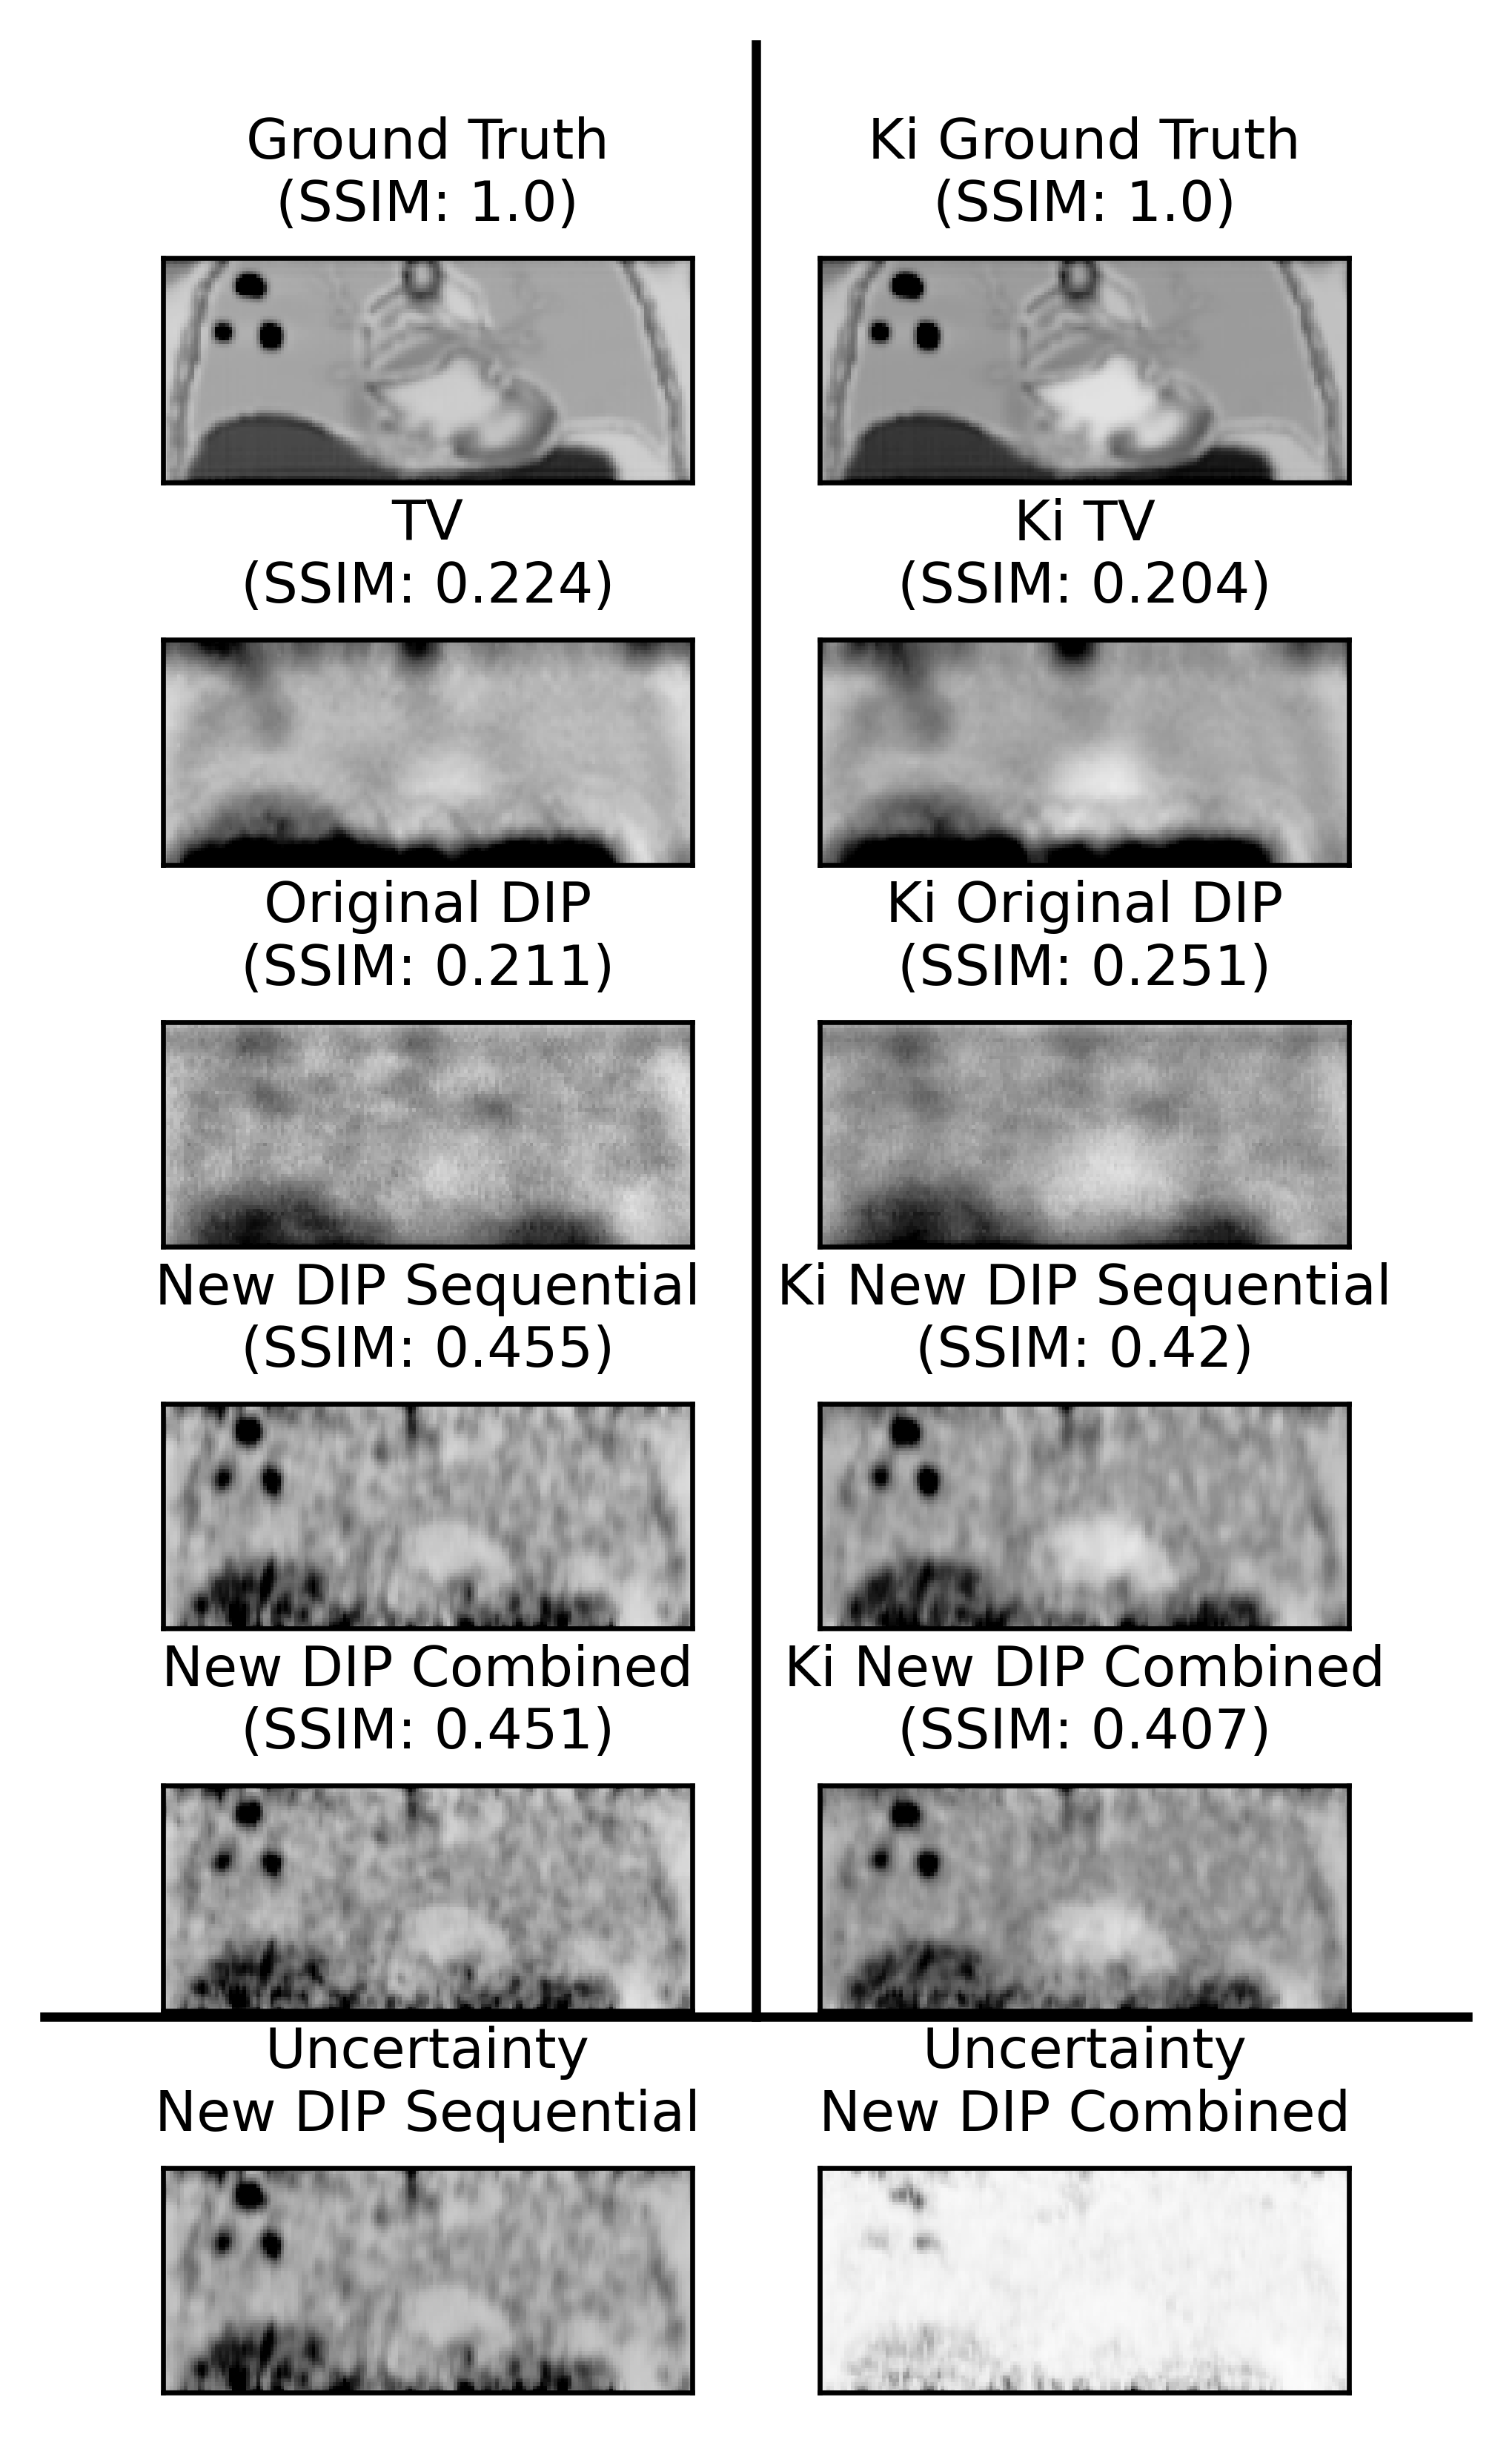
\includegraphics[width=0.9\linewidth]{visual_analysis.png}
                
                \begin{highlightbox}[UCLlightblue]
                    \captionsetup{singlelinecheck=false, justification=centering}
                    \caption{First row, first column denoised results, second column Ki results. Second row uncertainty results Colour map ranges consistent for all images in each section.}
                \end{highlightbox}
                
                \label{fig:visual_analysis}
            \end{figure}
            
            \begin{figure}[H]
                \centering
            
                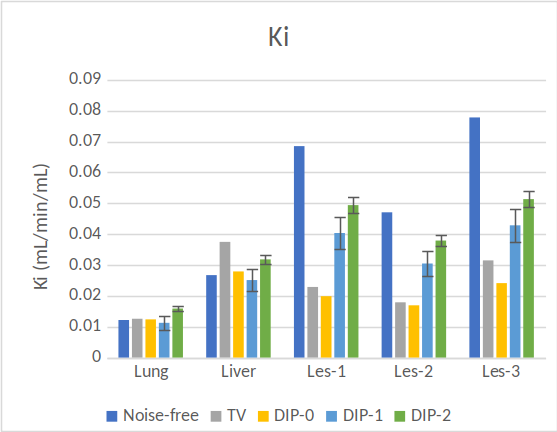
\includegraphics[width=0.9\linewidth]{ki.png}    
                
                \begin{highlightbox}[UCLlightblue]
                    \captionsetup{singlelinecheck=false, justification=centering}
                    \caption{Ki results (single voxel) of a Patlak reconstruction of all time points, plus uncertainty where applicable. \gls{DIP}-0 being the original, \gls{DIP}-1 being the new sequential, and \gls{DIP}-2 being the new combined implementation.}
                \end{highlightbox}
                
                \label{fig:ki}
            \end{figure}
    \end{multicols}
\end{document}
